\documentclass[titlepage,11pt]{article}
\usepackage{amsmath, amsthm, amssymb}
\usepackage{fullpage}
\usepackage{graphicx}
\usepackage{caption}
\usepackage{subcaption}
\usepackage{algorithmicx, algorithm}
\usepackage[noend]{algpseudocode}
\newcommand*\Let[2]{\State #1 $\gets$ #2}
\usepackage{float}
\usepackage{tikz}

\newtheorem{theorem}{Theorem}[section]


\begin{document}
\title{CoachRank}
\author{Akilesh Potti, Dominick Twitty, Wenhai Yang}
\maketitle


\tableofcontents

\section{Introduction}
Sports Illustrated, a magazine for sports enthusiasts, asks, "Who are the greatest college coaches, male or female, of the last century?" To answer this, we constructed a mathematical model to choose the top coaches in men's Basketball, men's Football, and men's Baseball. We also use these models to consider the difference between coaching in the past and in the present. Finally, we present an article for Sports Illustrated detailing our metrics and results at a non-technical level.

\section{Model Assumptions and Data Collection}
We make several assumptions in our modeling process:
\begin{itemize}
\item The idea of ``best all time college coach'' is subjective in nature, and to assess our model we have to focus more on qualitative assessment and justification, instead of a quantitative measure.

\item A coach's rank is determined and only determined by their achievement in the sport they coach, and is unrelated to other factors in their personal life.

\item The data we collect is considered true in all circumstances.
\end{itemize}

\subsection{Data Collection}
The accuracy and relevance of our results depended heavily on the quality and volume of data we could collect. That said, data collection was perhaps the most difficult part of our modeling process. We found that data on college sports is much harder to come by than data on professional sports. Within the scope of our search, less popular sports like Hockey simply did not have easily accessible data, especially from before 2001. We often found that when a site stated they had statistics on file, this meant that they had scanned copies of the original documents, which we could not parse.
\\

\noindent For what was available, we had to write web scrapers to collect the data in its human-readable format. This made collecting data on the largest scales time-prohibitive, even with generous caching and multithreading. Finally, we had to be mindful of the data use policies of our sources, and ensure that our collection methods used as little bandwidth as possible.
\\

\noindent We managed to collect a fair amount of data for Football, Basketball, and Baseball, the most popular college sports. All the data for these three sports were taken from Sports-Reference. For Basketball, we collected the career statistics for all coaches listed, back to 1895, for a total of over 3500 coaches. These statistics include total wins and losses, conference championships and appearances, and NCAA tournament statistics. We also collected per-school statistics for each coach. Finally, we collected the outcomes and point data for every NCAA tournament game. Aforementioned limitations prevented us from collecting outcome data for every regular season game. 
\\

\noindent We collected a similar scope of data for Football. We acquired career wins, losses, and bowl game statistics for every Football coach listed, back to 1877, for a total of over 2000 coaches. We also collected per-school statistics for each coach. Finally, we collected the outcomes and point data for every bowl game listed. Once again, time and data policies prevented us from collecting data on every game.
\\

\noindent For Baseball, we were only able to collect career statistics for about 100 coaches, each with over 1000 wins. That data was backed by a NCAA PDF that was presumably human-entered. Despite the huge gap in data volume, we chose Baseball because we could not find historical data on any level for the other sports listed.

\subsection{Coaches vs Teams}

One of the key assumptions we make in our approach is that in general, "best" coaches are largely independent of the team that they coach. This is a bold claim, but an important one as if this were true it allows us to simply analyze the coaches rather than the specific teams they coached and the players another way. Said another way, the mathematical models would be far more complex if the coaches and teams were tied together in terms of determining who is the "best coach". 
\\

\noindent We discuss the methodology used for testing this assumption for Basketball and for conserving space we don't discuss it for Football and Baseball. We test this assumption by observing the per-school statistics for each coach. For each (Coach, School) pair we have the percentage of games that the team won with that coach. From this dataset we know that if the coach has achieved approximately the same win percentage then we have strong reason to believe that the coaches and teams are independent enough to only construct the mathematical model around coach data without delving into player and team specific data. To test this formally, we use the Pearson chi squared statistical test to test if there is a discrete uniform distribution across the win percentage across all the teams coached. Out of the $3513$ basketball coaches, $755$ of them had coached more than one team in their career. Of these coaches, $87.6\%$ of them had a discrete uniform distribution across the number of win percentages, which largely says that we are fine in constructing mathematical models with just the coach data and not diving into the player data. We repeated similar statistical tests for football and found similar results.

\section{Models}

\subsection{Simple Win \& Loss Models}

We began with the simplest models and continually improved them. Naively, the most indicative measure of a coach's capability is the number of games won and the number of games lost, and this information is also easy to obtain. Therefore we started by considering different algorithms to rank coaches based only on their number of wins and losses.

\subsubsection{Sort by Win Percentage}
The simplest model involves computing the win percentage. That is, we score each coach by the ratio of wins to total games. This method has obvious flaws: it doesn't take into account the number of games played by the coaches: a coach with a 4-1 win-loss record is intuitively not better than a coach with a 100-70 record, though this model would say so.

\subsubsection{Sort by Net Wins}
Another simple model involves computing net wins. That is, we score each coach by wins minus losses. Intuitively, this takes into account the magnitude of the number of games won and lost. However, this can be shown to simply favor coaches who have played more games. 

\subsubsection{Sort by Scaled Win Ratio}
A third simple model involves multiplying the win ratio by the number of wins. This model is more robust than the previous two models because it takes into account both ratio of wins and losses and the magnitude. 

We subjectively considered the results produced by each of these model and decided that sorting by squared win and loss ratio produces the best results with no filtering of the data. This is the model we resort to given only career win and loss data.

\subsection{Graphical Model}
We had access to more data than career win and loss totals, and we incorporated connectivity data between coaches into a graph-based model. One can consider the nodes of the graph to be the coaches and the edges to represent relationships between pairs of coaches. Naturally, the edges between coaches in our graphs are based on games played between them. Depending on the situation, the edges could be weighted and/or directed either to or from the better coach.
\\

\noindent The main advantage of a graph-based approach is that it can observe direct interactions between pairs of coaches rather than considering coaches in isolation. It also allows us to apply transitivity to our data. That is, the relationship between two coaches can now be influenced by the pair's interactions with outside coaches. The approach even allows inferences about coach pairs who never played against each other by looking at paths in the graph. Therefore we can draw conclusions about coaches even though they came from different time periods.

\subsubsection{Topological Ordering}
The first idea that came to mind was to apply a topological ordering to the graph. That is, if we consider edges between pairs to point to the better coach, we want to remove coaches from the graph such that at time of removal, that coach has no incoming edges (and is therefore the worst coach). The idea is that the coach removed later would be the better.
\\

\noindent The major problem with this approach has to do with cycles. In order to construct a topological sort, we would either need a graph with no cycles (implying an already-existing partial order on coaches), or a mechanism for removing cycles from the graph. We could not create a satisfactory heuristic for removing cycles (that is, one that didn't seem too arbitrary).

\subsubsection{Markov Chain (CoachRank)}
Rather than a model that required we remove cycles from our graph, we decided it would be best to create a model that relied entirely on the structure of the graph created from the data.
\\

\noindent Imagine instead of having us, the spectators doing the voting and the ordering, each coach will have a $\bf{vote}$ of a certain $\bf{size}$, which the coach can divide up into pieces. The coach can then give the chunks of the vote to different coaches which she thinks is better than herself. We assume the coaches to be rational: the coach doesn't take into account the opinions of amateurs and public media, and she only gives out votes to the coaches who have beaten her. Then we will rank the coaches based on how many votes each coach eventually gets. Since the coaches form a graph in which there might be cycles, at each timestep a coach can be both receiving and giving votes. What we are interested in is the distribution of the votes in the long term.
\\

\noindent Consider the following example. There are four coaches: coach 1, coach 2, coach 3, coach 4. Coach 1 has been beaten by coaches 2 and 4, coach 2 has been beaten by coach 3 and coach 4, coach 3 has been beaten by coach 4 and coach 1, coach 4 has never been beaten.

\begin{center}
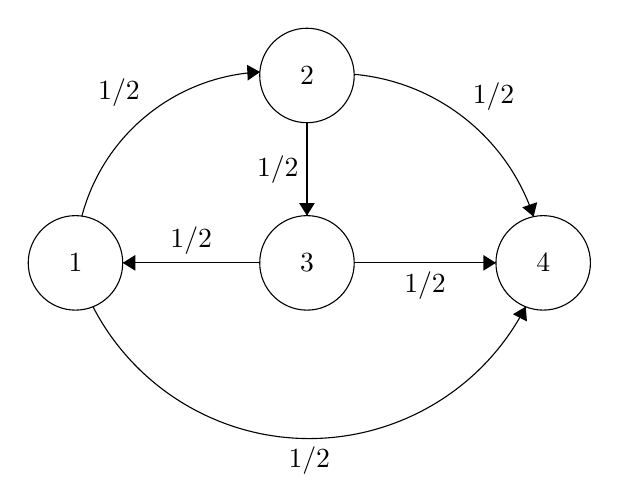
\begin{tikzpicture}[scale=0.2]
\tikzstyle{every node}+=[inner sep=0pt]
\draw [black] (37.8,-30.2) circle (3);
\draw (37.8,-30.2) node {$3$};
\draw [black] (23.1,-30.2) circle (3);
\draw (23.1,-30.2) node {$1$};
\draw [black] (37.8,-18.3) circle (3);
\draw (37.8,-18.3) node {$2$};
\draw [black] (52.8,-30.2) circle (3);
\draw (52.8,-30.2) node {$4$};
\draw [black] (51.691,-32.982) arc (-27.29025:-152.70975:15.462);
\fill [black] (51.69,-32.98) -- (50.88,-33.46) -- (51.77,-33.92);
\draw (37.95,-41.86) node [below] {$1/2$};
\draw [black] (23.506,-27.235) arc (165.22297:92.75902:12.309);
\fill [black] (34.82,-18.08) -- (33.99,-17.62) -- (34.04,-18.62);
\draw (25.86,-20.31) node [above] {$1/2$};
\draw [black] (40.793,-18.226) arc (84.9222:18.22552:13.234);
\fill [black] (52.19,-27.27) -- (52.42,-26.35) -- (51.47,-26.67);
\draw (49.65,-20.55) node [above] {$1/2$};
\draw [black] (34.8,-30.2) -- (26.1,-30.2);
\fill [black] (26.1,-30.2) -- (26.9,-30.7) -- (26.9,-29.7);
\draw (30.45,-29.7) node [above] {$1/2$};
\draw [black] (40.8,-30.2) -- (49.8,-30.2);
\fill [black] (49.8,-30.2) -- (49,-29.7) -- (49,-30.7);
\draw (45.3,-30.7) node [below] {$1/2$};
\draw [black] (37.8,-21.3) -- (37.8,-27.2);
\fill [black] (37.8,-27.2) -- (38.3,-26.4) -- (37.3,-26.4);
\draw (37.3,-24.25) node [left] {$1/2$};
\end{tikzpicture}
\end{center}

\noindent The Markov Chain above shows how the vote will be given out at each timestep: coach 1 will give out half of his vote to coach 2 and the other half to 3, coach 2 will give out half of her vote to coach 3 and the other half to coach 4, coach 3 will give out half of her vote to coach 1 and the other half to coach 4. Coach 4, since she never lost to anyone, will simply keep her vote to herself. This can be modeled as a Markov Chain, and the distribution of votes at some large time is the stationary probability distribution of this Markov Chain:

$$ \pi = \lim_{n \rightarrow \infty} \phi_{0} P^n \mbox{ for some initial distribution } \phi_{0}$$

\noindent where $\bf{P}$ is the probability transition matrix, with $\bf{P}_{i,j}$ equal to the proportion of coach i will give to coach j (can also be interpreted as the probability of going from i to j in the Markov Chain):

\[
\bf{P} = 
\begin{bmatrix}
0 & 0.5 & 0.5 & 0 \\
0 & 0 & 0.5 & 0.5 \\
0.5 & 0 & 0.5 & 0 \\
0 & 0 & 0 & 1
\end{bmatrix}
\]

\noindent We know that if the Markov Chain is irreducible and ergodic, then a stationary distribution exists and is unique. This is the left eigenvector of $\bf{P}$ for the eigenvalue 1.


\subsubsection*{Irreducible \& Ergodic}

\noindent The example we show doesn't satisfy the property because it's possible for coaches to be undefeated. To make sure the matrix we encounter will be irreducible and ergodic, we use a similar technique to the PageRank algorithm used by Google:

\begin{enumerate}
\item For dead-ends (coach 4 in the example), in each step she will split her vote into equal pieces and give one piece to every coach, (go to a random state in the Markov Chain)
\item For non-dead-ends (coach 1, 2, 3 in the example), in each step with he will first split her vote into two, with proportion $\alpha$ and $1 - \alpha$. With the $\alpha$ proportion she did what she did before, spliting it and give the pieces to coaches who have beaten her, the remaining $1 - \alpha$ she will split into equal pieces and give one piece to every coach.
\end{enumerate}

\noindent Therefore, after adjusting for deadends in ${\bf P}$, the new probability transition matrix can be represented as:

$${\bf D} = \alpha {\bf P} + (1 - \alpha) {\bf U}$$

\noindent where $\bf{U}$ with all entries equal to $\frac{1}{n}$, $n$ being the total number of coaches (or number of states in the Markov Chain).
\\

\noindent With the new probability transition matrix, since all entries in $\bf{D}$ are positive, we know by Perron-Frobenius theorem that $\bf{D}$ is both irreducible and ergodic, and that the stationary distribution $\pi$ exists and is unique. With $\pi$ we can find the coaches with the top $5$ probability and they will be the "best" college coaches of all time since they get the most proportion of votes from all coaches in the long-run.

\subsubsection*{Formal Representation}

$$G(V, E) \mbox{ represents the graph of coaches}$$
$$V = \{v_1, v_2 ... v_n\} \mbox{ where } v_i \mbox{ is coach i }$$
$$(v_i, v_j) \in E : \mbox{ coach j beats coach i more often than coach i beats coach j }$$



\[
    {\bf P} (i, j)= 
\begin{cases}
    \frac{ I_{\{(v_i, v_j) \in E\}}}{d(v_i)},& \text{if } d(v_i) \geq 1\\
    \frac{1}{n},              & \text{otherwise}
\end{cases}
\]

$${\bf D} (i, j) = \alpha {\bf P} (i, j)  + (1-\alpha)\frac{1}{n}$$


\subsubsection*{Efficient Implementation}


Since the matrix ${\bf D}$ is huge and all entries are non zero, calculating its eigenvalues and eigenvectors directly can be very inefficient computationally. However ${\bf P}$ is a sparse matrix and most of its entries are zero. To make sure we will be able to produce the eigenvector that represents the stationary distribution efficiently, we use Power Method:

\vspace{5mm}

\begin{algorithm}[H]
\begin{algorithmic}
\State{$v = (1/n, ... ,1/n)$}
\While{$\| \alpha v {\bf P} + (1 - \alpha)(1, ... ,1) - v\|_2 < e^{-8}$}
\State{$v = \alpha v {\bf P} + (1 - \alpha)(1, ... ,1)$}
\EndWhile
\Return{$v$}
\end{algorithmic}
\end{algorithm}

\vspace{5mm}

\noindent Since $v {\bf P}$ can be calculated using sparse matrix ${\bf P}$, this algorithm is much more computationally efficient than simply calculating the eigenvectors of ${\bf D}$. As $\alpha$ increases, the time it takes for $v$ to converge is shorter, but the difference in the ranking might be less significant, therefore this is a tradeoff and we pick $\alpha = 0.95$.

\subsubsection*{Edge Weights}

\noindent In the model we introduced above, in situations where $d(v_i) \geq 1$, ${\bf P}(i, j) = \frac{ I_{\{(v_i, v_j) \in E\}}}{d(v_i)}$. However there is a lot more information we can capture:

\begin{enumerate}
\item Importance of the game: The more important the game is, the game result will be more informative, and more likely coach $i$ will be to give the vote to coach $j$.
\item Career: If it is early in the career of coach $i$ when he lost to coach $j$, she is going to put less weight than the game she lost later in her career, since it is typical for a coach to learn from failure early and become a better coach later. Therefore coach $i$ will be more convinced to give vote to someone she lost to later in her career.
\item Game Score: A close game is less convincing than a game entirely dominated by an opponent. Therefore the more points coach $i$ lost, the more convinced she will be to give her vote to her opponent.
\end{enumerate}

\noindent There is more information we can obtain; however, due to the difficulty of data collection, we come up with the following updated formula to calculate the weight for edge weight:
\\

\noindent Let $T$ be the set of all games
\\
$f: T \rightarrow \mathbb{R}$ maps a game to the score difference of the game (positive winning score, 0 if draw)
\\
$h: T \rightarrow \mathbb{I}$ returns the importance multiplier of a game, it is sport specific since different sport have different game structure.
\\
$\beta: $ the score difference adjustment, it is specific to a type of sport.

$$ T_{i,j} = \{t \in T : \mbox{ coach i lost to coach j in } t\} $$
$$w(v_i, v_j) =  \max(0, \sum_{t \in T_{i, j}} h(t) \log(1 + \beta f(t)) - \sum_{t \in T_{j, i}} h(t) \log(1 + \beta f(t))) $$
$$(v_i, v_j) \in E \mbox{ if } w(v_i, v_j) > 0$$

\[
    {\bf P}(i, j)= 
\begin{cases}
    \dfrac{w(v_i, v_j)}{\sum_{w(v_i, v_k) > 0} w(v_i, v_k)},      & \text{if } d(v_i) \geq 1\\
    \frac{1}{n},              & \text{otherwise}
\end{cases}
\]
\\

\noindent The intuition for this formula is really straightforward: for example, if a coach lost 30 points in championship game, it definitely is going matter much more than a loss of 4 points in an early-season game. The weight for an edge is a combination of the two factors: the importance of the game and the score difference.

\subsubsection*{Parameter Estimation}
\noindent $h:$ we let $h = (\text{number of games of a given importance})^{-1}$. The reason for this approximation is clear, the less frequent a type of sub-game is, the more it is valued. Say for example that a team  playes 30 regular season games, 5 tournament games, and 1 championship game, then $h(\mbox{season}) = 1/30$, $h(\mbox{tournament}) = 1/5$, $h(\mbox{championship}) = 1$. Similarly, in college Football, $h(\mbox{season}) = 1/12$, $h(\mbox{playoff}) = 1/12$, $h(\mbox{championship}) = 1$
\\

\noindent Let $\beta:$ be the inverse of the median of score differences of a sport in the data. From the data, we calculated the median and set $\beta_{basketball} = \frac{1}{9}$, $\beta_{football} = \frac{1}{10}$. We do not use the mean because there are outliers in the score difference distribution, as we can see in the following graph:
\\

\begin{figure}[H]
      \centering
      \begin{subfigure}{0.48\textwidth}
      \caption{Distribution of Basketball Score Difference}
      \centering
      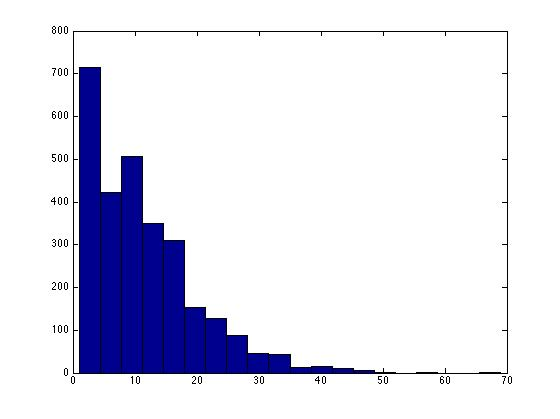
\includegraphics[width=1.1\textwidth]{graphs/basketball_diff_dist.jpg}
      \end{subfigure}\quad
      \begin{subfigure}{0.48\textwidth}
      \caption{Distribution of Football Score Difference}
      \centering
      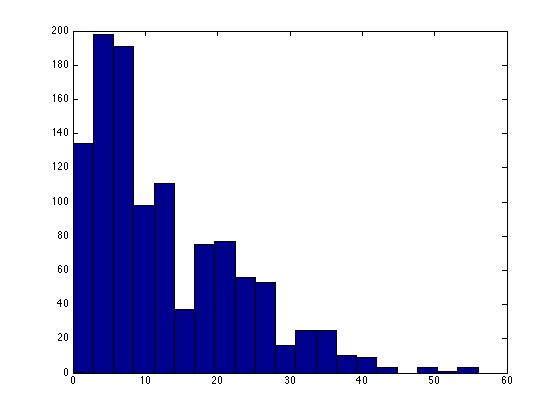
\includegraphics[width=1.1\textwidth]{graphs/football_diff_dist.jpg}
      \end{subfigure}
 \end{figure}

\noindent 
\\

\noindent There are a lot more possible variations with edge weights in the graphical model. However, as more detailed information is added into the model, the less significant it is, especially among the top results returned. Therefore due to time constraints the above model and method of parameter estimation is the final version we decided to use for our graphical model. As we can see in the results and validation section, the results are promising.

\subsection{Machine Learning Model}

\noindent So far we have algorithms that produce the top 5 "best coaches" according to historical data, but we could also interpret "best" as who has the best chance of winning in the future, or is overall "best" looking forward. Additionally, it is difficult to assess the CoachRank graphical model or more importantly figure out what attributes of a coach are the most important for defining "best coach". There are a lot of sports fans who may not understand the whole graphical model, but can understand certain key attributes of coaches. This leads us to the use of machine learning methods for tackling this unsupervised learning problem- we found significant difficulty finding structure within the massive amounts of sports data, but we realized that the CoachRank graphical model posed above can bring \textit{structure} to formulate a supervised learning problem. Furthermore, we can use variable selection methods to extract out which are the most important attributes for deciding who the best coach is. 

\subsubsection*{Feature Correlation}

\noindent Before we start to use machine learning methods, it's important to get a feel for the data to make sure the models we produce are intuitively sound. After the initial data munging phase, we realized that a lot of the attributes (now on refered to as features) were correlated, which made sense because our data sets had wins, losses, total games played, etc. To make it the most interpretable and simplest model, we removed features that had a high degree of correlation. Below is the Pearson correlation matrix for basketball: 

\begin{figure}[H]
      \caption{Pearson Correlation matrix for basketabll features}
      \centering
      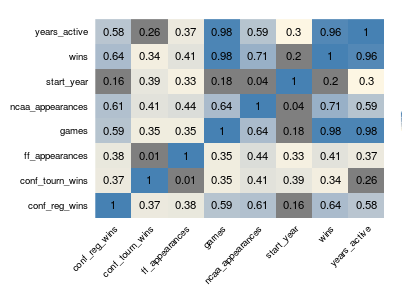
\includegraphics[width=1.0\textwidth]{bball_cor.jpg}
\end{figure}

\noindent From the matrix above, we can clearly see that there are some attributes (wins, losses, games, etc.) that are colored dark blue, which we removed moving forward to create a compact set of features that explained what constituted as the "best coach" without redundancy. There are a wealth of supervised machine learning methods that we can use, but we have two defined goals: figure out what features make up the best coach and assess how well the graphical model works. To best achieve these goals, we decided to use multiple linear regression to figure out how each feature correlates with the coach's CoachRank value. This is also easy to explain to sports fans.

\subsubsection*{Multiple Linear Regression}

Multiple Linear Regression is a supervised machine learning method that predicts a real valued output given a set of features. More formally, the multiple linear regression function is:

\begin{center}
$E[CoachRankValue|X] = \gamma + \sum_{i=0}^{n} X_{i}$
\end{center}

\noindent That is, we are finding the conditional expectation of the CoachRank value of a coach given a set of features $X$. Since we would not only like to predict CoachRank values for coaches but also individually analyze the features, we handled multicollinearity by using the Pearson correlation matrix above to ensure none of the features were correlated above a minimum threshold of $0.9$. We also looked at the distribution of the features to make sure the homoscedasticity, weak exogeneity, and independence assumptions of linear regression held true. Once we performed the analysis, we observed the plots of the residuals to ensure that they were in fact normally distributed as that's another major assumption of regerssion. Below are the results of the multiple linear regression model:

\begin{center}
\begin{tabular}{ | c | c |}
\hline
Features            & Coefficients \\\hline
conf_reg_wins       & -0.02572      \\\hline
conf_tourn_wins     & 0.24730     \\\hline
ff_appearances      &  1.47954    \\\hline
ncaa_appearances    & 0.24730      \\\hline
games               & 0.00210      \\
\hline
\end{tabular}
\end{center}

\vspace{2 mm}

\noindent The features that were statistically significant at the highest threshold were $ncaa-appearances$ and $ff-appearances$, which intuitively make sense and in fact are used in the construction of the CoachRank graphical model. Additionally, the sign of the features make sense as the more final four and NCAA appearances a coach has the more popular or "good" they are likely to be. What's not intuitive is the real-valued coefficients of the features, and the number of features that we have: does one feature "predict" the CoachRank value of the coach better than other features? That is commonly referred to as variable selection, where there currently exist a wealth of methods. We use least-angle regression (LARS) for computing which features best correlate with the CoachRank. In a nutshell, LARS intializes all the coefficients of the features at zero and takes the largest step in the direction of the most correlated variable with CoachRank, until some other feature is more correlated, at which point LARS proceeds in a equiangular direction to both features, hence the name "least-angle". At the end of the day, LARS provides us which features that are the most "important" in determining the CoachRank values. The plot is shown below:

\begin{figure}[H]
      \caption{LARS of Basketball Features}
      \centering
      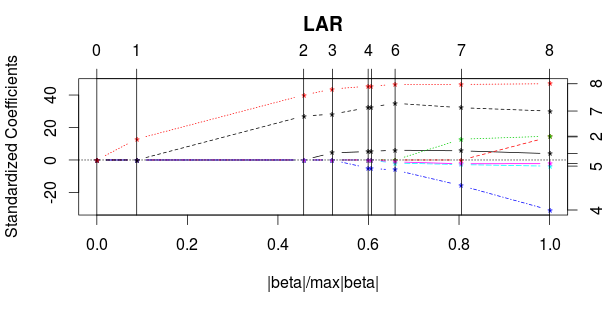
\includegraphics[width=1.0\textwidth]{bball_lars.jpg}
\end{figure}

\noindent As expected, the $ncaa-appearances$ and $ff-appearances$ enter first and are thus deemed to be the most "important". Now it remains to figure out how to make the coefficients of the features more interpretable in a way that sports fans can understand it. Fortunately, intereptable models in supervised learning are a growing area of research within predictive modeling and machine learning. In the next section we discuss a natural extension to the multiple linear regression model discussed above known as Supersparse Linear Integer Models, which one of the group members is currently working on with Professor Cynthia Rudin at MIT, so are able to use the code although it's not publicly released yet.

\subsubsection*{Supersparse Linear Integer Model}

Supersparse Linear Integer Models (SLIM) create predictive scoring systems that are both practical and interpretable. They are widely refered to as intrepretable models because they require users to perform only a few operations to make a prediction. They further restrict the coefficients to a certain set of integral values so that we can better understand the effect of the features on the predicted value. SLIM is formulated as a mixed integer program with an objective function that minimizes 0-1 training loss and $L_0$ and $L_1$ norm to ensure both accuracy, sparsity, and interpretability respectively. Although this is a computationally hard problem (NP-Hard), due the size of our data set and CPLEX solver from IBM we are able to obtain results within a reasonable amount of time. Additionally, as this is a classification model, we had to have a surjective mapping of our real valued CoachRank values to discrete buckets ($<0.01$, $>0.02$, etc). Since we had a imbalanced data set that resulted, that is the number of coaches falling into each bucket varied widely, we used the imbalanced formulation of SLIM. After doing so, we obtained results that, as expected, are close to the results of our multiple linear regression model but now have integral values for the features.        

\subsubsection*{Can we abstract this?}

\noindent Okay, so we have these neat supervised machine learning methods that complement the complicated graphical CoachRank algorithm that we discussed earlier- so what? Well, the purpose of the machine learning methods was two fold: one to extract features from the CoachRank graphical model to actually determine how it's figuring out which coaches are the "best" and two to understand how these features interact with each other and affect the CoachRank value in a practical and interpretable way, both of which were done through the multiple linear regression model and supersparse linear integer model discussed above.  

\vspace{2 mm}

\noindent A natural question that one may now ask is first how can we extend this trained machine learning models to other time periods and other genders. Well, a nice feature about both the graphical model and the supervised learning model is that they are specifically constructed for specific sports: sure, they might have inputs as "final four appearances" or "bowl games", but almost every sport has major competitions and team games that can be substituted for this. Additionally, not where in either model do we construct the model on any gender specific criteria, so our assumption is that these models above will hold for both genders \textit{assuming} both genders have similar abstract characteristics, which we believe at a first order approximation to be true. As far as different time periods go for the machine learning method, we partitioned the coaches into different data sets depending on their start year and found that the most significant extracted features were in fact largely the same, which is no surprise because there should not be a significant difference between the most important features that determine the best coach between different time periods. However, it is important to note we noticed in earlier time periods (1913-1940), there were less features that were found as statistically significant which might mean that the notion of "best" coach was more simplistic way back when but now has grown more complicated in determining what constitutes as the "best" coach as the game and society has evolved: an interesting observation.    


\section{Results \& Validation}

\subsection{Result of Graphical Model (CoachRank)}

Using the Markov Chain model with the edge weight function that takes game's importance, and score difference into account, we computed the following result and showed the top five coaches for Male College Football and Male College Basketball:

\subsubsection*{Male College Football}

\noindent The graph $G(V, E)$ for Male College Football have 529 nodes, 1032 edges, and 27 weakly connected components. The fact that there is no one single connected component is possibly due to the small size of our dataset. The top five coaches are:

\begin{center}
\begin{tabular}{ | c | c | }
\hline
Coach Name   & Vote \% \\\hline
Joe Paterno  & 0.02421 \\\hline
Mack Brown   & 0.01728 \\\hline
Bear Bryant  & 0.01663 \\\hline
Lloyd Carr   & 0.01491 \\\hline
Pete Carroll & 0.01338 \\
\hline
\end{tabular}
\end{center}

\subsubsection*{Male College Basketball}

\noindent The graph $G(V, E)$ for Male College Basketball have 763 nodes, 2582 edges, and 1 weakly connected component. The fact that $G$ is weakly connected is really useful in that it allow us to compare every two coaches in the graph, even though they are playing in different time horizon. The top five coaches are:

\begin{center}
\begin{tabular}{ | c | c | }
\hline
Coach Name  & Vote \% \\\hline
Mike Krzyzewski & 0.03272 \\\hline
Dean Smith  & 0.02544 \\\hline
Roy Williams & 0.02329 \\\hline
John Wooden  & 0.02170 \\\hline
Rick Pitino  & 0.02066 \\
\hline
\end{tabular}
\end{center}

\subsubsection*{Male College Baseball}

Due to the lack of connectivity data between baseball coaches, we resort to sorting by scaled win ratio.
\begin{center}
\begin{tabular}{ | c | c | c| c | }
\hline
Coach Name       & $w (w / w + l)$ \\\hline
Ed Cheff         & 1361.60 \\\hline
Gene Stephenson  & 1343.38 \\\hline
Mike Martin      & 1316.73 \\\hline
Augie Garrido    & 1279.37 \\\hline
Gordie Gillespie & 1259.56 \\
\hline
\end{tabular}
\end{center}

\noindent If we plot the Vote \% of all the College Basketball coaches from high to low, we can get the following histogram. Similar graphs were computed for Baseball and Football.

\begin{figure}[H]
      \caption{Male College Basketball Vote \%}
      \centering
      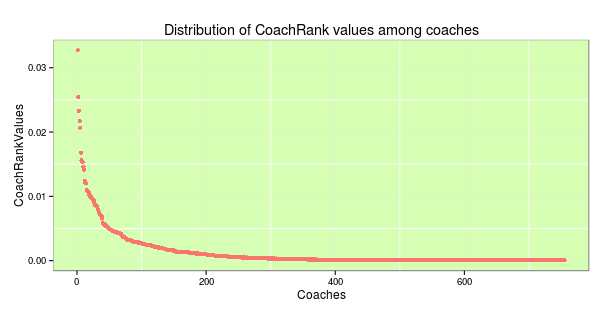
\includegraphics[width=1\textwidth]{graphs/basketball_score_dist.png}
 \end{figure}

\noindent We find some very interesting facts from this graph:

\begin{enumerate}
\item The curves drop off very quickly, which means there are large differences between coaches with the top votes.
\item A small proportion of coaches hold the majority of the votes. In Male College Basketball, $5.6\%$ of the coaches hold $50\%$ of the votes. In Male College Football, $12.4\%$ of the coaches hold $50\%$ of the votes.
\end{enumerate}

\subsubsection*{Comparison Across Time Horizon}

If we plot the vote \% of all the College Basketball coaches over the start year of their careers, we can get the following histogram:

\begin{figure}[H]
      \caption{Vote \% Distribution over Career Start Year}
      \centering
      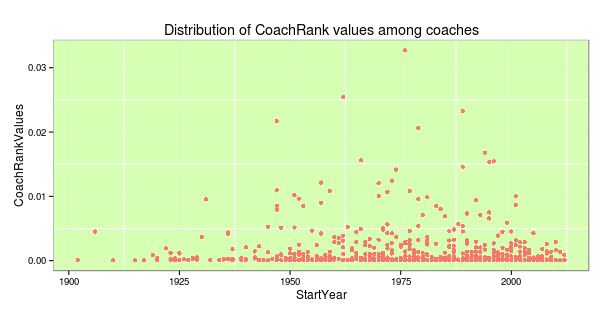
\includegraphics[width=1\textwidth]{graphs/time_horizon.png}
 \end{figure}

\noindent We can see from the graph that the scores of the coaches have a positive correlation with the start-year of their career. This is reasonbale because first techniques of sports tend to improve overtime and second due to the shortage of data for earlier periods we have more connectivity for coaches in later periods in the graphical model.
\\

\noindent We also run the graphical model in separate time periods, and the results for the different periods (1900-1930, 1930-1970, 1970-2010) are reasonable baed on information from public polls and professional sports media.

\subsubsection*{Applying the Model to Other Sports}

Applying the graphical model to other sports are very straightforward. First obtain enough data of games played between coaches, the scores of the games, and the importance of the games. Then adjust $\beta$ and $h$ based on the median score difference and league structure. With this information we can run the graphical model and calculate vote \% for each coach and select the top 5 results as the "best college coaches of all time".

\subsubsection*{Assessment}

\noindent Due to the subjective nature of this problem, assessment of the results can be tricky. By comparing both of our results with public polls and professional sports media such as ESPN and Fox News, etc., and looking at the achievements of the top coaches, we conclude that the result is consistent with public opinions.

\subsubsection*{Robustness}

\noindent Varying parameters $\alpha$ from 0.75 to 0.95, and scaling $\beta$ upwards and downwards by $10\%$, the top 5 coaches returned doesn't have much difference, just with minor rank movement among the top 10 coaches. This is in part due to the quick drop-off rate of the curves above, and the large score differences between top coaches. Therefore, we conclude that the result of the graphical model is valid and it is robust to small perturbations in parameters.

\section{Strengths and Weaknesses}

\subsection{Strengths}
\begin{itemize}
\item The graphical model allows us to be more objective in our ranking algorithm since we can understand it as the coaches voting among themselves based on their game history, instead of arbitrary tweaking of heuristics.

\item We take into account not only the career data of a coach, but also the game result, game score, and the game importance of the games they play against each other.

\item We have an efficient implementation of using the power method to calculate the stationary distribution of the Markov Chain, and the results show clear differentiation between coaches, especially high-ranking ones.
\end{itemize}

\subsection{Weaknesses}
\begin{itemize}
\item Due to the limited amount of data we could collect, we could not consider coaches not in our dataset. For example, John Gagliardi, the coach with the most wins in college Football history, was not in our data set because he competed in the NAIA and NCAA Division III leagues. 

\item Our graphical model used only postseason games as input. We justify this heuristically by saying that only skilled coaches will be play in the postseason. However, this produces somewhat sparse graphs, especially compared to those we could have generated if we were able to collect data on every game.

\item Assessment is also difficult since ranking is in itself subjective. Our methods of assessment are limited to public polls, professional sport media, coaches' achievements, and cross-validation between our different models.

\end{itemize}

\section{Conclusions}
With the graphical model, the top 5 coaches for Male College Football are Joe Paterno, Mack Brown, Bear Bryant, Lloyd Carr, Pete Carroll. The top 5 coaches for Male College Basketball are Mike Krzyzewski, Dean Smith, Roy Williams, John Wooden, Rick Pitino. The top 5 coaches for Male College Baseball are Ed Cheff, Mike Martin, Gene Stephenson, Augie Garrido, Gordie Gillespie.

\section{Future work}
\begin{itemize}
\item Obtain more game data and coach career information, and more information about the coaches to train a better model.

\item Come up with an objective mechanism to assess the result of our ranking, such as incorporating more public sources.

\item Control for more variables such as home/away, team players etc. in our model, and apply the model to more sports.
\end{itemize}

\pagebreak

\section{Bibliography}
\begin{thebibliography}{9}

\bibitem{Pagerank} Pagerank Algorithm,
\verb|http://ilpubs.stanford.edu:8090/422/1/1999-66.pdf|
\bibitem{Re} $\text{A stochastic optimization model for real-time ambulance redeployment}$,
\\\verb|http://www.sciencedirect.com/science/article/pii/S0305054813000385|
\bibitem{Ithaca} Ithaca Demographics,
\verb|http://www.ci.ithaca.ny.us/maps/index.cfm|
\bibitem{Cornell} Cornell Demographics,
\verb|http://www.cornell.edu/about/facts/stats.cfm|
\bibitem{IC} Ithaca College,
\verb|http://www.ithaca.edu/admission/facts/|


\end{thebibliography}

\end{document}
